\documentclass[aps,prf,preprint,groupedaddress]{revtex4-2}
\usepackage[utf8]{inputenc}
\usepackage[svgnames,dvipsnames]{xcolor}
\usepackage[T1]{fontenc}
\usepackage{tikz}
\usetikzlibrary{shapes.geometric,calc}
\usetikzlibrary{shapes}
\usepackage{pgfplots}
\usepackage{amsmath,amsfonts,amssymb}
\usepackage{colortbl}
\usepackage[colorlinks=false,linkcolor=blue ,filecolor=red ]{hyperref}

\begin{document}

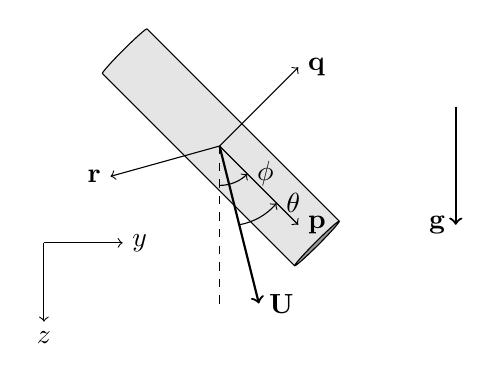
\begin{tikzpicture}[scale=1.]
\node[cylinder, 
    draw = black, 
    text = black,
    cylinder uses custom fill, 
    cylinder body fill = black!10, 
    cylinder end fill = black!40,
    aspect = 0.2, 
    shape border rotate = 90, rotate =225, minimum height=3.5cm, minimum width=0.8cm] (c) at (2,2,2) {};


\draw[->] (2,2,2)   -- (3,1,2) node [at end, right]   {$\mathbf{p}$};
\draw[->] (2,2,2)   -- (3,3,2) node [at end, right]   {$\mathbf{q}$};
\draw[->] (2,2,2)   -- (1,2,3) node [at end, left]   {$\mathbf{r}$};


\draw[->, thick] (2,2,2)--(2.5,0,2) node[right]{$\mathbf{U}$};

\draw[-, dashed] (2,2,2)--(2,0,2);

\draw[->] (2.25,1,2) arc (-80:-40:0.8)node[right]{$\theta$};
\draw[->] (2,1.5,2) arc (-90:-45:0.5)node[right]{$\phi$};
\draw[->, thick] (5,2.5,2)--(5,1,2) node[left]{$\mathbf{g}$};


\draw[->] (-1,0,0)--(-1,-1,0)node[below]{$z$};
\draw[->] (-1,0,0)--(0,0,0)node[right]{$y$};

\end{tikzpicture}

\end{document}